\mfpicnumber{1}

\opengraphsfile{Parabolas}

\setcounter{footnote}{0}

\label{Parabolas}

We begin our study of the conic sections with parabolas, since we have already seen parabolas described as graphs of quadratic functions,  $f(x) = ax^2 + bx + c$ ($a \neq 0$).  It turns out that we can also describe parabolas in terms of distances.

\medskip

\colorbox{ResultColor}{\bbm

\begin{defn}

\label{paraboladefn}

Let $F$ be a point in the plane and $D$ be a line not containing $F$.   A \index{parabola ! definition of}  \textbf{parabola} is the set of all points equidistant from $F$ and $D$.  The point $F$ is called the \textbf{focus} \index{parabola ! focus} \index{focus (foci) ! of a parabola} of the parabola and the line $D$ is called the \textbf{directrix} \index{parabola ! directrix} \index{directrix ! of a parabola} of the parabola. 

\end{defn}

\ebm}

\medskip

Schematically, we have the following.

\begin{center}

\begin{mfpic}[15]{-7}{7}{0}{5}
\dashed \polyline{(0,2), (0,0), (0,-2)}
\dashed \polyline{(0,2), (2, 0.5), (2, -2)}
\dashed \polyline{(0,2), (-2,0.5), (-2, -2)}
\dashed  \polyline{(0,2), (4,2), (4, -2)}
\dashed  \polyline{(0,2), (-4,2), (-4, -2)}
\dashed \polyline{(0,2), (6,4.5), (6, -2)}
\dashed  \polyline{(0,2), (-6,4.5), (-6, -2)}
\plotsymbol[3pt]{Asterisk}{(0, 2)}
\tlabel[cc](6.5, -2.5){$D$}
\tlabel[cc](0, 2.5){$F$}
\arrow \reverse \arrow \function{-6.5, 6.5, 0.1}{-2}
\penwd{1.25pt}
\arrow \reverse \arrow \function{-6.25,6.25,0.1}{(x**2)/8}
\point[4pt]{(0,0)}
\point[4pt]{(2,0.5)}
\point[4pt]{(-2,0.5)}
\point[4pt]{(4,2)}
\point[4pt]{(-4,2)}
\point[4pt]{(6,4.5)}
\point[4pt]{(-6,4.5)}
\tlabel[cc](0.5,-0.5){$V$}
\end{mfpic}

\end{center}

Each dashed line from the point $F$ to a point on the curve has the same length as the dashed line from the point on the curve to the line $D$.  The point suggestively labeled $V$ is, as you may expect, the \textbf{vertex}.  The \index{parabola ! vertex} \index{vertex ! of a parabola} vertex is the point on the parabola closest to the focus.  

\smallskip

We want to use only the distance definition of parabola to derive the equation of a parabola and, if all is right with the universe, we should get an expression much like those studied in Section \ref{QuadraticFunctions}.  


\smallskip

For simplicity, assume that the vertex is $(0,0)$ and that the parabola opens upwards.  Let $p$ denote the directed\footnote{We'll talk more about what `directed' means later.} distance from the vertex to the focus, which by definition is the same as the distance from the vertex to the directrix.   Hence, the focus is $(0,p)$ and the directrix is the line $y = -p$.  Our picture becomes 

\begin{center}

\begin{mfpic}[15]{-7}{7}{0}{5}
\axes
\plotsymbol[3pt]{Asterisk}{(0, 2)}
\tlabel[cc](0.75, 1.5){$(0,p)$}
\tlabel(7,-0.25){\scriptsize $x$}
\tlabel(0.25,5){\scriptsize $y$}
\arrow \reverse \arrow \function{-6.5, 6.5, 0.1}{-2}
\tlabel[cc](0, -2.5){$y = -p$}
\tlabel[cc](7, 3.75){$(x,y)$}
\dashed \polyline{(0,2), (6, 4.5), (6, -2)}
\tlabel[cc](6, -2.5){$(x, -p)$}
\tlabel[cc](0.5,-0.5){$(0,0)$}
\penwd{1.25pt}
\arrow \reverse \arrow \function{-6.25,6.25,0.1}{(x**2)/8}
\point[4pt]{(6, -2)}
\point[4pt]{(0,0)}
\point[4pt]{(6,4.5)}
\end{mfpic}

\end{center}

From the definition of parabola, we know the distance from $(0,p)$ to $(x,y)$ is the same as the distance from $(x,-p)$ to $(x,y)$.  Using the Distance Formula, Equation \ref{distanceformula}, we get

\[ \begin{array}{rclr} \sqrt{(x -0)^2 + (y-p)^2} & = & \sqrt{(x-x)^2 + (y - (-p))^2} & \\
\sqrt{x^2 + (y-p)^2} & = & \sqrt{(y+p)^2} & \\
x^2 + (y-p)^2 & = & (y+p)^2 & \mbox{square both sides} \\
x^2 + y^2 - 2py + p^2 & = & y^2 + 2py + p^2 & \mbox{expand quantities} \\
x^2 & = & 4py & \mbox{gather like terms} \\ \end{array} \]

Solving for $y$ yields $y = \frac{x^2}{4p} = \frac{1}{4p} x^2$, which is a quadratic function of the form found in Equation \ref{vertexofquadraticfunctions} with $a = \frac{1}{4p}$ and vertex $(0, 0)$.


\smallskip

We know from previous experience that if the coefficient of $x^2$ is negative, the parabola opens downwards.  In the equation $y = \frac{1}{4p} x^2$ this happens when $p < 0$.  In our formulation, we say that $p$ is a `directed distance' from the vertex to the focus:  if $p > 0$, the focus is above the vertex;  if $p < 0$, the focus is below the vertex.   The \index{parabola ! focal length} \index{focal length of a parabola} \textbf{focal length} of a parabola, that is, the length from the vertex to the focus,  is therefore $|p|$.


\smallskip

If we choose to place the vertex at an arbitrary point $(h,k)$, we arrive at the following formula  using either transformations from Section \ref{Transformations} or re-deriving the formula from Definition \ref{paraboladefn}.

\medskip

\colorbox{ResultColor}{\bbm

\begin{eqn}  \label{standardvparabola} \index{parabola ! standard equation ! vertical}  \textbf{The Standard Equation of a Vertical\footnote{That is, a parabola which opens either upwards or downwards.}  Parabola in the $xy$-plane:}  

The equation of a (vertical) parabola with vertex $(h,k)$ and focal length $|p|$ is

\[ (x-h)^2 = 4p(y-k) \]

If $p>0$, the parabola opens upwards;  if $p < 0$, it opens downwards.
  
\end{eqn}
  
\ebm}
  
\medskip

Notice that in the standard equation of the parabola above, only one of the variables, $x$, is squared. As we'll see in the coming sections, this is a quick way to distinguish the equation of a parabola from equations representing the other conic sections.

\smallskip

Before embarking on an example,  we take a moment to better illustrate the affect of the focal length  $|p|$ on the graph of a parabola.  Below we sketch three parabolas with focal length $0.5$, $1$, and $2$.  In each case, the focus is denoted by an `$\ast$.'  In general, as the focal length $|p|$ increases, the parabola becomes wider.

\begin{center}

\begin{tabular}{m{1.5in}m{2in}m{3in}}

\begin{mfpic}[15]{-3}{3}{0}{5}
\plotsymbol[3pt]{Asterisk}{(0, 0.5)}
\tcaption{$p = 0.5$}
\tlabel[cc](0, 1.5){$F$}
\dashed \polyline{(-1,0.5), (1,0.5)}
\tlabel[cc](0,-0.5){$V$}
\penwd{1.25pt}
\arrow \reverse \arrow \function{-3,3,0.1}{(x**2)/2}
\point[4pt]{(0,0), (-1,0.5), (1,0.5)}
\end{mfpic}

&

\begin{mfpic}[15]{-5}{5}{0}{5}
\plotsymbol[3pt]{Asterisk}{(0, 1)}
\tcaption{$p = 1$}
\tlabel[cc](0, 1.5){$F$}
\dashed \polyline{(-2,1), (2,1)}
\tlabel[cc](0,-0.5){$V$}
\penwd{1.25pt}
\arrow \reverse \arrow \function{-4.2,4.2,0.1}{(x**2)/4}
\point[4pt]{(0,0), (2,1), (-2,1)}
\end{mfpic}

&

\begin{mfpic}[15]{-7}{7}{0}{5}
\plotsymbol[3pt]{Asterisk}{(0, 2)}
\tcaption{$p = 2$}
\tlabel[cc](0, 1.5){$F$}
\dashed \polyline{(-4,2), (4,2)}
\tlabel[cc](0,-0.5){$V$}
\penwd{1.25pt}
\arrow \reverse \arrow \function{-6.2,6.2,0.1}{(x**2)/8}
\point[4pt]{(0,0), (4,2), (-4,2)}
\end{mfpic}

\\

\end{tabular}

\end{center}

The dashed line segment in each of the illustrations above is called the \textit{latus rectum} of the parabola.  More specifically, the \index{parabola ! latus rectum} \index{latus rectum of a parabola}\textbf{latus rectum} of a parabola is the line segment with endpoints on the parabola which contains the focus and is parallel to the directrix.\footnote{Hence, the endpoints of the latus rectum are  two points on `opposite' sides of the parabola.}   


\smallskip

We leave it to the reader to show  that the length of the latus rectum, called the \index{parabola ! focal diameter} \index{focal diameter of a parabola} \textbf{focal diameter} of the parabola is $|4p| = 4|p|$, which appears ever so conveniently in the standard form as stated in Equation \ref{standardvparabola}.  


\smallskip

Knowing the focus and focal diameter allows to plot two points on the parabola in addition to the vertex, thus producing a more accurate graph.

\begin{ex} \label{verticalparabolaex} $~$

\begin{enumerate}

\item  Graph  $(x+1)^2 = -8(y-3)$ in the $xy$-plane.  Find the vertex, focus, and directrix.  State the focal length, focal diameter, and find the endpoints of the latus rectum.

\item  Find the standard form of the equation of the parabola with focus $(2,1)$ and directrix $y = -4$.

\item  Find the standard form of the equation of the parabola sketched below:

\begin{center}

\begin{mfpic}[15]{-5}{5}{-5}{5}
\axes
\xmarks{-4, -3, -2, -1, 0, 1, 2, 3, 4}
\ymarks{-4,-3,-2,-1,0,1,2,3,4}
\tlabel(5,-0.5){\scriptsize $x$}
\tlabel(0.5,5){\scriptsize $y$}
\tlabel[cc](-1.5, 2.5){\scriptsize $(-1,2)$}
\tlabel[cc](1.5,0.5){\scriptsize $(1,0)$}
\tlpointsep{4pt}
\scriptsize
\axislabels {x}{ {$-4 \hspace{7pt}$} -4,  {$-2 \hspace{7pt}$} -2, {$-1 \hspace{7pt}$} -1, {$2$} 2,   {$3$} 3, {$4$} 4}
\axislabels {y}{ {$3$} 3,  {$4$} 4, {$-1$} -1, {$-2$} -2, {$-3$} -3, {$-4$} -4}
\normalsize
\penwd{1.25pt}
\arrow \reverse \arrow \function{-4.5,2.5,0.1}{2-(0.5)*((x+1)**2)}
\point[4pt]{(-1,2), (1,0)}
\end{mfpic}

\end{center}

\end{enumerate}

\medskip

{\bf Solution.}  

\begin{enumerate}

\item  Rewriting $(x+1)^2 =  -8(y-3)$ as $(x-(-1))^2 =  -8(y-3)$,  we identify $h = -1$ and  $k = 3$ in  Equation \ref{standardvparabola},  so the vertex is $(-1,3)$.  Additionally, we have $4p = -8$ so $p = -2$.  Since $p < 0$, the focus is  \textit{below} the vertex so the parabola opens \textit{downwards}.  


\smallskip

The focal length is $|p| = 2$, which means the focus is $2$ units below the vertex.  From $(-1,3)$, we move down $2$ units and find the focus at $(-1,3-2) = (-1,1)$.  Likewise the directrix is $2$ units above the vertex, or the horizontal line $y=3+2 = 5$.  



\smallskip

The focal diameter is $|4p| = |-8| = 8$, which means the parabola is $8$ units wide at the focus.  Hence, the endpoints of the latus rectum are $4$ units to the left and right of the focus.  Starting at $(-1,1)$ and moving to the left $4$ units, we arrive at $(-1-4,1) = (-5,1)$.  Starting at $(-1,1)$ and moving to the right $4$ units we arrive at $(-1+4,1) = (3,1)$.  The final graph appears below on the left.


\smallskip


\item We begin by sketching the data given to us below on the right.   Since the focus is $(2,1)$, we know the the vertex lies on the vertical line $x=2$.  Moreover, since the vertex is halfway between the focus and directrix, we know the vertex is exactly $\frac{5}{2}$ units \textit{below} the focus at $\left(2,1-\frac{5}{2} \right) = \left(2, -\frac{3}{2} \right)$.  This gives $h=2$ and $k = -\frac{3}{2}$.  Since the focus of the parabola is $\frac{5}{2}$ units \textit{above} the vertex we know  $p = + \frac{5}{2}$.  Using  Equation \ref{standardvparabola}, we get our final answer:  $(x-2)^2 = 4 \left(\frac{5}{2}\right) \left(y - \left(- \frac{3}{2}\right) \right)^2$ or  $(x-2)^2 = 10 \left(y + \frac{3}{2}\right)^2$.


\begin{center}

\begin{multicols}{2}

\begin{mfpic}[15]{-7}{5}{-1}{6}
\axes
\xmarks{-6, -5, -4, -3, -2, -1, 0, 1, 2, 3, 4}
\ymarks{0, 1, 2, 3, 4, 5}
\dashed \polyline{(-5,1), (3,1)}
\plotsymbol[3pt]{Asterisk}{(-1,1)}
\tlabel(5,-0.25){\scriptsize $x$}
\tlabel(0.25,6){\scriptsize $y$}
\tlabel[cc](-5.5,1.5){\scriptsize $(-5,1)$}
\tlabel[cc](-1.5,3.5){\scriptsize $(-1,3)$}
\tlabel[cc](3.5,1.5){\scriptsize $(3,1)$}
\tlabel[cc](1.5, 4.5){\scriptsize $y=5$}
\tcaption{\scriptsize The graph of $(x+1)^2 = -8(y-3)$}
\arrow \reverse \arrow \function{-7,5,0.1}{5}
\tlpointsep{4pt}
\scriptsize
\axislabels {x}{ {$-5 \hspace{7pt}$} -5, {$-4 \hspace{7pt}$} -4, {$-3 \hspace{7pt}$} -3, {$-2 \hspace{7pt}$} -2, {$-1 \hspace{7pt}$} -1, {$1$} 1, {$2$} 2,  {$3$} 3}
\axislabels {y}{{$1$} 1, {$2$} 2}
\normalsize
\penwd{1.25pt}
\arrow \reverse \arrow \function{-6.5,4.5,0.1}{((x+1)**2)/-8+3}
\point[4pt]{(-1,3), (3,1), (-5,1)}
\end{mfpic}


\begin{mfpic}[15]{-2}{4}{-5}{2}
\axes
\xmarks{-1,0,1,2,3}
\ymarks{-4,-3,-2,-1,0,1}
\tlabel(4,0.25){\scriptsize $x$}
\tlabel(0.25,2){\scriptsize $y$}
\tcaption{\vphantom{\scriptsize The graph of $(x+1)^2 = -8(y-3)$}}
\arrow \reverse \arrow \function{-1,4,0.1}{-4}
\dashed \polyline{(2,1), (2, -4)}
\plotsymbol[4pt]{Asterisk}{(2,1)}
\point[4pt]{(2,-1.5)}
\tlpointsep{4pt}
\scriptsize
\axislabels {x}{{$-1 \hspace{7pt}$} -1, {$1$} 1, {$2$} 2, {$3$} 3}
\axislabels {y}{{$-3$} -3, {$-2$} -2, {$-1$} -1, {$1$} 1}
\normalsize
\end{mfpic}

\end{multicols}


\end{center}

\item  From the graph, we assume the point labeled $(-1,2)$ is the vertex, which means in the context of  Equation \ref{standardvparabola}, $h = -1$ and $k = 2$.  Hence, at this point, we know the equation is $(x-(-1))^2 = 4p (y-2)$, or, more simply $(x+1)^2 = 4p(y-2)$.  


\smallskip

To determine the value of $p$, we see $(1,0)$ is on the graph so when $x = 1$, $y = 0$.  Substituting these values into our equation gives $(1+1)^2 = 4p(0-2)$ so $4=-8p$ or $p = -\frac{1}{2}$.  (The fact $p<0$ tracks with the parabola opening downwards.)  Hence, $4p = 4\left( -\frac{1}{2} \right) = -2$ so the equation of the parabola is  $(x+1)^2 = -2(y-2)$.  We leave it to the reader to check our answer analytically and graphically. \qed 

\end{enumerate}

\end{ex}

We can produce `horizontal' parabolas in the $xy$-plane by reflecting our so-called `vertical' parabolas about the line $y=x$.  As you may recall from Section \ref{InverseFunctions}, we accomplish this algebraically by interchanging the variables $x$ and $y$.  Such parabolas necessarily open to the left or to the right, which means that unlike the vertical parabolas, these parabolas do not represent $y$ as a function of $x$.   As we shall see, however, they can \textit{implicitly} describe $y$ as a function of $x$, provided certain restrictions are in place.

\medskip

\colorbox{ResultColor}{\bbm

\begin{eqn}  \label{standardhparabola} \index{parabola ! standard equation ! horizontal} \textbf{The Standard Equation of a Horizontal Parabola:}  

The equation of a (horizontal) parabola with vertex $(h,k)$ and focal length $|p|$ is

\[ (y-k)^2 = 4p(x-h) \]

If $p>0$, the parabola opens to the right;  if $p < 0$, it opens to the left.
  
\end{eqn}
  
\ebm}
  
\medskip

As we saw in  Section \ref{InverseFunctions}, when we reflect a horizontal line across the line $y=x$, we obtain a vertical line, and, as a result, the directrix of a \textit{horizontal} parabola is a \textit{vertical} line. Moreover, the focus of a horizontal parabola is either to the \textit{left} or \text{right} of the directrix.  Schematically:

\begin{center}

\begin{tabular}{m{2.5in}m{2.5in}}

\begin{mfpic}[13]{0}{5}{-7}{7}
\plotsymbol[3pt]{Asterisk}{(-2, 0)}
\tlabel[cc](-2.5, 0){$F$}
\arrow \reverse \arrow \parafcn{-6.5, 6.5, 0.1}{(2,t)}
\tlabel[cc](2.5, 6.5){$D$}
\tlabel[cc](0.5,0){$V$}
\penwd{1.25pt}
\arrow \reverse \arrow \parafcn{-6.25,6.25,0.1}{-((t**2)/8,t)}
\point[4pt]{(0,0)}
\end{mfpic}

&


\begin{mfpic}[13]{0}{5}{-7}{7}
\plotsymbol[3pt]{Asterisk}{(2, 0)}
\tlabel[cc](2.5, 0){$F$}
\arrow \reverse \arrow \parafcn{-6.5, 6.5, 0.1}{(-2,t)}
\tlabel[cc](-2.5, 6.5){$D$}
\tlabel[cc](-0.5,0){$V$}
\penwd{1.25pt}
\arrow \reverse \arrow \parafcn{-6.25,6.25,0.1}{((t**2)/8,t)}
\point[4pt]{(0,0)}
\end{mfpic}

 \\

$p< 0$ 

&



$p>0$ \\


\end{tabular}

\end{center}



\begin{ex} \label{horizontalparabolaex}  $~$

\begin{enumerate} 

\item \label{hparabolaeqnex1} For each of the equations below:

\begin{itemize}

\item  Graph the equation in the $xy$-plane.

\item  Find the vertex, focus, and directrix.  State the focal length, focal diameter, and find the endpoints of the latus rectum.

\end{itemize}

\begin{multicols}{2}

\begin{enumerate}

\item $(y-2)^2 = 12(x+1)$. 

\item \label{ctsparabolaex} $y^2 + 4y + 8x = 4$

\end{enumerate}

\end{multicols}

\item  Represent each of the parabolas in number \ref{hparabolaeqnex1} as the graphs of two or more explicit functions of $x$.

\item  Find the standard form of the parabola satisfying the following characteristics:

\begin{enumerate}

\item  The focus is $(-4,2)$ and the directrix is the $y$-axis.

\item  The parabola whose graph is sketched below:

\begin{center}

\begin{mfpic}[15]{-5}{5}{-2}{8}
\axes
\xmarks{-4, -3, -2, -1, 0, 1, 2, 3, 4}
\ymarks{-1,0,1,2,3,4,5,6,7}
\tlabel(5,-0.5){\scriptsize $x$}
\tlabel(0.5,8){\scriptsize $y$}
\tlabel[cc](-3.5, 3){\scriptsize $(-2,3)$}
\tlabel[cc](-0.75,-0.75){\scriptsize $(0,0)$}
\tlabel[cc](-1, 6){\scriptsize $(0,6)$}
\tlpointsep{4pt}
\scriptsize
\axislabels {x}{ {$-4 \hspace{7pt}$} -4, {$-3 \hspace{7pt}$} -3, {$-2 \hspace{7pt}$} -2, {$2$} 2,   {$3$} 3, {$4$} 4}
\axislabels {y}{ {$1$} 1,  {$2$} 2, {$3$} 3, {$4$} 4, {$5$} 5,  {$7$} 7}
\normalsize
\penwd{1.25pt}
\arrow \reverse \arrow \parafcn{-2,8,0.1}{(   (((t-3)**2)/4.5) - 2, t)}
\point[4pt]{(0,0),  (-2,3), (0,6)}
\end{mfpic}

\end{center}

\end{enumerate}


\end{enumerate}

\medskip

{\bf Solution.} 


\begin{enumerate}

\item

\begin{enumerate}

\item  Rewriting $(y-2)^2 = 12(x+1)$ as $(y-2)^2 = 12(x-(-1))$, we identify $h=-1$ and $k=2$ so per  Equation \ref{standardhparabola}, the vertex is $(-1,2)$.  We also see that $4p = 12$ so $p = 3$.  Since $p>0$, this means the focus is to the \textit{right} of the vertex so the parabola opens to the \textit{right}.


\smallskip

The focal length is $|p| = 3$, which means the focus is $3$ units to the right of the vertex.  From $(-1,2)$, we move  $3$ units to the right and find the focus at $(-1+3,2) = (2,2)$.  Likewise the directrix is $3$ units to the left of the vertex, the vertical  line $x=-1-3 = -4$.  


\smallskip

The focal diameter is $|4p| = |12| = 12$, which means the parabola is $12$ units wide at the focus.  Hence, the endpoints of the latus rectum are $6$ units above and below  the focus.  Starting at $(2,2)$ and moving down $6$ units, we arrive at $(2,2-6) = (2,-4)$.  Starting at $(2,2)$ and moving up  $6$ units we arrive at $(2,2+6) = (2,8)$.  The final graph appears below on the left.

\item  Unlike the previous example, the equation  $y^2 + 4y + 8x = 4$ is not in the form described  in Equation \ref{standardhparabola}.  In order to get an equivalent equation in the form prescribed by  Equation \ref{standardhparabola}, we need to complete the square in $y$  on the left-hand side of the equation.  Once that is done, we  factor out the coefficient of $x$ on the other side of the equation below.

\[ \begin{array}{rclr} y^2+4y+8x &  = & 4 & \\
y^2 + 4y &  = & -8x + 4 &  \\
y^2+4y+4 & = & -8x+4+4 & \mbox{complete the square in $y$.} \\
(y+2)^2 & = &-8x+8 & \mbox{factor}  \\ 
(y+2)^2 & = & -8(x-1) &   \end{array} \]

The equation $(y+2)^2 = -8(x-1)$, rewritten as $(y-(-2))^2 = -8(x-1)$ is in the form given in Equation \ref{standardhparabola}.  Identifying  $h = 1$ and $k = -2$, we get the vertex is $(1,-2)$.  Moreover, we see $4p = -8$ so that $p = -2$.  The fact that $p < 0$, means the focus will be the \textit{left} of the vertex so the parabola will open to the \textit{left}.  


\smallskip


Since the focal length is  $|p| = 2$, the focus is $2$ units to the left of the vertex.   From $(1,-2)$ and move left $2$ units and arrive at the focus $(1-2,-2) = (-1,-2)$.  Similarly, the directrix is $2$ units to the right of the vertex, the vertical line $x=1+2 = 3$.  


\smallskip

Since the focal diameter is $|4p|$ is $8$, the parabola is $8$ units wide at the focus.  Starting at the focus $(-1,-2)$ we move down $4$ units and get $(-1,-2-4) = (-1,-6)$.  Moving up $4$ units from the focus we get $(-1,-2+4) = (-1,2)$.  Hence, $(-1,-6)$ and $(-1,2)$ are the endpoints of the latus rectum. The final graph appears below on the right.

\pagebreak

\begin{center}

\begin{multicols}{2}

\begin{mfpic}[15][10]{-6}{4}{-5}{9}
\axes
\arrow\polyline{(-4,-5),(-4,9)}
\arrow\polyline{(-4,9),(-4,-5)}
\xmarks{-5,-4,-3, -2,-1,0,1,2,3}
\ymarks{-4,-3,-2,-1,0,1,2,3,4,5,6,7,8}
\tlabel(4,-0.25){\scriptsize $x$}
\tlabel(0.25,9){\scriptsize $y$}
\tcaption{\scriptsize The graph of $(y-2)^2 = 12(x+1)$}
\plotsymbol[3pt]{Asterisk}{(2,2)}
\tlpointsep{4pt}
\scriptsize
\axislabels {x}{{$-5 \hspace{7pt}$} -5, {$-4 \hspace{7pt}$} -4, {$-3 \hspace{7pt}$} -3, {$-2 \hspace{7pt}$} -2, {$-1 \hspace{7pt}$} -1, {$1$} 1, {$2$} 2, {$3$} 3}
\axislabels {y}{{$-4$} -4, {$-3$} -3, {$-2$} -2, {$-1$} -1, {$1$} 1, {$2$} 2, {$3$} 3, {$4$} 4, {$5$} 5, {$6$} 6, {$7$} 7, {$8$} 8}
\normalsize
\penwd{1.25pt}
\arrow \reverse \arrow \parafcn{-4.5,8.5,.1}{(((t-2)**2)/12-1,t)}
\point[4pt]{(2,8), (2,-4), (-1,2)}
\end{mfpic}



\begin{mfpic}[15]{-3}{4}{-7}{3}
\axes
\arrow\polyline{(3,3),(3,-7)}
\arrow\polyline{(3,-7),(3,3)}
\xmarks{-2,-1,0,1,2,3}
\ymarks{-6,-5,-4,-3,-2,-1,0,1,2}
\tlabel(4,-0.25){\scriptsize  $x$}
\tlabel(0.25,3){ \scriptsize $y$}
\tcaption{\scriptsize The graph of $y^2 + 4y + 8x = 4$}
\plotsymbol[3pt]{Asterisk}{(-1,-2)}
\tlpointsep{4pt}
\scriptsize
\axislabels {x}{{$-2 \hspace{7pt}$} -2, {$-1 \hspace{7pt}$} -1, {$1$} 1, {$2$} 2}
\axislabels {y}{{$-6$} -6, {$-5$} -5, {$-4$} -4, {$-3$} -3, {$-2$} -2, {$-1$} -1, {$1$} 1, {$2$} 2}
\normalsize
\penwd{1.25pt}
\arrow \parafcn{-6.5,2.5,.1}{((4-t**2-4*t)/8,t)}
\arrow \parafcn{2.5,-6.5,.1}{((4-t**2-4*t)/8,t)}
\point[4pt]{(1,-2), (-1,2), (-1,-6)}
\end{mfpic}

\end{multicols}

\end{center}

\end{enumerate}

\item To describe these parabolas as graphs of functions of $x$, we solve each equation for $y$ in terms of $x$.  

\begin{enumerate}

\item Starting with $(y-2)^2 = 12(x+1)$, we extract square roots to get $y - 2 = \pm \sqrt{12(x+1)}$.   Isolating $y$, we get   $y = 2 \pm \sqrt{12(x+1)}$ which simplifies to $y = 2 \pm 2 \sqrt{3x+3}$.  


\smallskip

We let $f(x) = 2 + \sqrt{3x+3}$ and $g(x) = 2-\sqrt{3x+3}$. Note that since $\sqrt{3x+3} \geq 0$ by definition, $f(x) = 2 + \sqrt{3x+3} \geq 2$ which means the graph of $f$ describes the \textit{upper} half of the parabola.  Similarly, the graph of $g(x) = 2 - \sqrt{3x+3}$ describes the \textit{lower} half of the parabola.


\smallskip

\item We can solve $y^2 + 4y + 8x = 4$ for $y$ by completing the square or using the quadratic formula.  We leave the former to the reader,\footnote{The standard form of the parabola will make an appearance using this route.} and proceed with the latter for the sake of practice.


\smallskip

To use the quadratic formula, we need to set the equation to $0$:  $y^2 + 4y + 8x-4 = 0$.  Since we are solving for $y$, we identify $a = 1$, $b=4$ and $c = 8x-4$.  We find the discriminant $b^2-4ac = (4)^2 - 4(1)(8x-4) = 32-32x$ so \[ y = \dfrac{-4 \pm \sqrt{32-32x}}{2} = \dfrac{-4 \pm \sqrt{32(1-x)}}{2}  = \dfrac{-4 \pm 4\sqrt{2(1-x)}}{2} = -2 \pm 2 \sqrt{2-2x}. \]

We identify $f(x) =  -2 + 2 \sqrt{2-2x}$ and $g(x) =  -2 - 2 \sqrt{2-2x}$. Since $\sqrt{2-2x} \geq 0$, we see the graph of $f$ traces out the \textit{upper} half of the parabola while the graph of $g$ traces out the \textit{lower} half of the parabola.

\end{enumerate}

\item  

\begin{enumerate}

\item  We sketch the data below.  Since the focus is $(-4,2)$ and the directrix is a vertical line, we know the vertex must lie on the horizontal line $y = 2$.  Moreover, we know the vertex must lie midway between the focus and directrix which in this case is  $(-2,2)$.  This gives $h = -2$ and $k = 2$.  Since the focus is $2$ units to the \textit{left} of the vertex, we know $p = -2$.  Using  Equation \ref{standardhparabola}, we get our answer as $(y-2)^2 = 4(-2)(x-(-2))$ or $(y-2)^2 = -8(x+2)$.


\begin{center}
\begin{mfpic}[15]{-5}{2}{-1}{4}
\axes
\xmarks{-4, -3, -2, -1, 0}
\ymarks{1,2,3}
\dashed \polyline{(-4,2), (0,2)}
\plotsymbol[3pt]{Asterisk}{(-4,2)}
\tlabel(2,-0.5){\scriptsize $x$}
\tlabel(0.5,4){\scriptsize $y$}
\tlabel[cc](-4, 1.5){\scriptsize $(-4,2)$}
\tlpointsep{4pt}
\scriptsize
\axislabels {x}{ {$-4 \hspace{7pt}$} -4, {$-3 \hspace{7pt}$} -3, {$-2 \hspace{7pt}$} -2, {$-1 \hspace{7pt}$} -1}
\axislabels {y}{ {$1$} 1,  {$2$} 2, {$3$} 3}
\normalsize
\penwd{1.25pt}
\arrow \reverse \arrow \polyline{(0,-1), (0,4)}
\end{mfpic}
\end{center}

\item  From the graph, we may infer the vertex of the parabola is $(-2,3)$ so $h = -2$ and $k = 3$.  Per Equation \ref{standardhparabola}, we have $(y-3)^2 = 4p(x-(-2))$ or $(y-3)^2 = 4p(x+2)$.  Since the graph contains $(0,6)$, we substitute $x=0$ and $y=6$ to get $(6-3)^2 = 4p(0+2)$.  We find $p = \frac{9}{8}$ which gives our final answer $(y-3)^2 = 4\left( \frac{9}{8} \right) (x+2)$ or $(y-3)^2 = \frac{9}{2} (x+2)$. \qed


\end{enumerate}

\end{enumerate}

\end{ex}

As we have seen, not all equations which describe parabolas will immediately match Equation \ref{standardvparabola} or Equation \ref{standardhparabola}.  Indeed, completing the square as we did with the equation in number \ref{ctsparabolaex} in Example \ref{horizontalparabolaex}  will be a necessary skill not only in this section, but in the rest of this chapter. 

\smallskip

 For parabolas, we summarize the procedure for putting an equation of a parabola into standard form below.  Of key importance is that in the equation for a parabola, one, and only one, of the variables are squared.

\smallskip

\colorbox{ResultColor}{\bbm

\centerline{\textbf{To Write the Equation of a Parabola in Standard Form}}

\begin{enumerate}

\item  Group the variable which is squared on one side of the equation and position the non-squared variable and the constant on the other side.

\item  Complete the square if necessary and divide by the coefficient of the perfect square.

\item  Factor out the coefficient of the non-squared variable from it and the constant.

\end{enumerate}

\ebm}

\smallskip

\phantomsection
\label{paraboloid}
In studying quadratic functions, we have seen parabolas used to model physical phenomena such as the trajectories of projectiles.  Other applications of the parabola concern its \index{parabola ! reflective property}`reflective property' which necessitates knowing about the focus of a parabola.  For example, many satellite dishes are formed in the shape of a \index{paraboloid} \textbf{paraboloid of revolution} as depicted below.

\begin{center}

\begin{tabular}{cc}

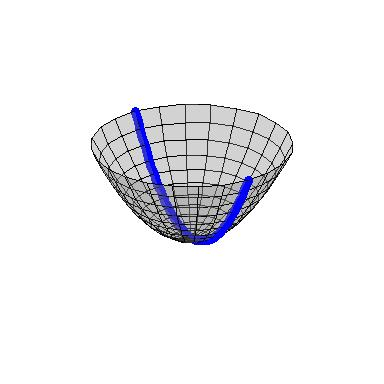
\includegraphics[width=2.5in]{./ParabolasGraphics/Paraboloid01.jpg} & 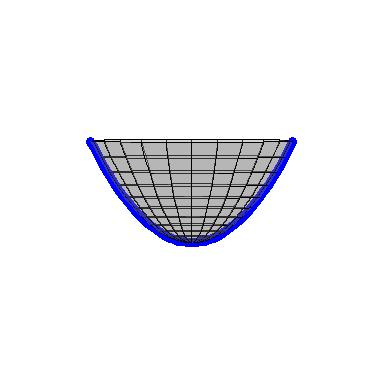
\includegraphics[width=2.5in]{./ParabolasGraphics/Paraboloid02.jpg} \\

\end{tabular}

\end{center}

Every cross section through the vertex of the paraboloid is a parabola with the same focus.  To see why this is important, imagine the dashed lines below as electromagnetic waves heading towards a parabolic dish.   It turns out that the waves reflect off the parabola and concentrate at the focus which then becomes the optimal place for the receiver. 

\smallskip

If, on the other hand, we imagine the dashed lines as emanating from the focus, we see that the waves are reflected off the parabola in a coherent fashion as in the case in a flashlight.  Here, the bulb is placed at the focus and the light rays are reflected off a parabolic mirror to give directional light.

\begin{center}

\begin{mfpic}[15]{-5}{7}{-1}{10}
\arrow \reverse \arrow \rotatepath{(0,0), -45}  \function{-6.25,6.25,0.1}{(x**2)/8}
\dashed  \rotatepath{(0,0), -45}   \polyline{(0,2), (2, 0.5), (2, 6)} 
\dashed  \rotatepath{(0,0), -45} \polyline{(0,2), (-2,0.5), (-2, 6)}
\dashed \rotatepath{(0,0), -45}   \polyline{(0,2), (4,2), (4, 6)}
\dashed \rotatepath{(0,0), -45}   \polyline{(0,2), (-4,2), (-4, 6)}
\dashed \rotatepath{(0,0), -45}  \polyline{(0,2), (6,4.5), (6, 6)}
\dashed \rotatepath{(0,0), -45}  \polyline{(0,2), (-6,4.5), (-6, 6)}
\plotsymbol[3pt]{Asterisk}{(1.414, 1.414)}
\tlabel[cc](2, 2){$F$}
\gfill \rotatepath{(0,0), -45}  \circle{(2,0.5),0.07}
\gfill \rotatepath{(0,0), -45}  \circle{(-2,0.5),0.07}
\gfill \rotatepath{(0,0), -45}  \circle{(4,2),0.07}
\gfill \rotatepath{(0,0), -45}  \circle{(-4,2),0.07}
\gfill \rotatepath{(0,0), -45} \circle{(6,4.5),0.07}
\gfill \rotatepath{(0,0), -45} \circle{(-6,4.5),0.07}
\end{mfpic}

\end{center}

\begin{ex} A satellite dish is to be constructed in the shape of a paraboloid of revolution.  If the receiver placed at the focus is located 2 ft above the vertex of the dish, and the dish is to be 12 feet wide, how deep will the dish be?

\smallskip

{\bf Solution.}  One way to approach this problem is to determine the equation of the parabola suggested to us by this data.  For simplicity, we'll assume the vertex is $(0,0)$ and the parabola opens upwards.  Our standard form for such a parabola is $x^2 = 4py$.  Since the focus is $2$ units above the vertex, we know  $p=2$, so we have $x^2 = 8y$.  Visually,

\begin{center}

\begin{mfpic}[25]{-7}{7}{0}{5}
\axes
\xmarks{-6, -5, -4, -3, -2, -1, 0,1,2,3,4,5,6}
\ymarks{0,1,2,3,4}
\arrow \polyline{(-5.5, 4.5),(5.5,4.5)}
\arrow \polyline{(5.5,4.5), (-5.5, 4.5)}
\arrow \polyline{(6, 0.5),(6,4)}
\arrow \polyline{(6,4), (6,0.5)}
\plotsymbol[3pt]{Asterisk}{(0, 2)}
\tlabel[cc](6.25,2.25){?}
\tlabel(6.25, 4.25){$(6,y)$}
\tlabel(0.25,5){$y$}
\tlabel(7, -0.25){$x$}
\gclear \tlabelrect[cc](0,4){$12$ units wide}
\tlpointsep{4pt}
\small
\axislabels {x}{{$-6 \hspace{7pt}$} -6, {$6$} 6}
\axislabels {y}{{$2$} 2}
\normalsize
\penwd{1.25pt}
\arrow \function{-6.25,6.25,0.1}{(x**2)/8}
\arrow \function{6.25,-6.25,0.1}{(x**2)/8}
\point[4pt]{(0,0), (6,36/8), (-6,36/8)}
\end{mfpic}

\end{center}

Since the parabola is $12$ feet wide, we know the edge is $6$ feet from the vertex.  To find the depth, we are looking for the $y$ value when $x=6$.  Substituting $x=6$ into the equation of the parabola yields $6^2 = 8y$ or $y = \frac{36}{8} = \frac{9}{2} = 4.5$.  Hence, the dish will be  $4.5$ feet deep.  \qed

\end{ex}

\newpage

\subsection{Exercises}

\label{ExercisesforParabolas}

In Exercises \ref{parabolasketchfirst} - \ref{parabolasketchlast},  graph of the given equations in the $xy$-plane.  Find the vertex, focus and directrix.  Include the endpoints of the latus rectum in your sketch.

\begin{multicols}{2}
\begin{enumerate}

\item $(x - 3)^{2} = -16y$ \label{parabolasketchfirst}
\item $\left(x + \frac{7}{3}\right)^{2} = 2\left(y + \frac{5}{2}\right)$


\setcounter{HW}{\value{enumi}}
\end{enumerate}
\end{multicols}

\begin{multicols}{2}
\begin{enumerate}
\setcounter{enumi}{\value{HW}}


\item \label{paranotfcnone} $(y - 2)^{2} = -12(x + 3)$ 
\item  \label{paranotfcntwo} $(y + 4)^{2} = 4x$

\setcounter{HW}{\value{enumi}}
\end{enumerate}
\end{multicols}

\begin{multicols}{2}
\begin{enumerate}
\setcounter{enumi}{\value{HW}}


\item $(x-1)^2 = 4(y+3)$
\item $(x+2)^2 = -20(y-5)$


\setcounter{HW}{\value{enumi}}
\end{enumerate}
\end{multicols}

\begin{multicols}{2}
\begin{enumerate}
\setcounter{enumi}{\value{HW}}

\item \label{paranotfcnthree} $(y-4)^2 = 18(x-2)$
\item  \label{paranotfcnfour} $\left(y+ \frac{3}{2}\right)^2 = -7 \left(x+ \frac{9}{2}\right)$ \label{parabolasketchlast}


\setcounter{HW}{\value{enumi}}
\end{enumerate}
\end{multicols}


In Exercises \ref{stdfrmparabolafirst} - \ref{stdfrmparabolalast}, put the equation into standard form.  Find the vertex, focus and directrix.\footnote{\ldots assuming the equation were graphed in the $xy$-plane.}

\begin{multicols}{2}
\begin{enumerate}
\setcounter{enumi}{\value{HW}}

\item  \label{paranotfcnfive} $y^{2} - 10y - 27x + 133 = 0$ \label{stdfrmparabolafirst}
\item $25x^{2} + 20x + 5y - 1 = 0$

\setcounter{HW}{\value{enumi}}
\end{enumerate}
\end{multicols}

\begin{multicols}{2}
\begin{enumerate}
\setcounter{enumi}{\value{HW}}

\item $x^2 + 2x - 8y + 49 = 0$
\item  \label{paranotfcnsix} $2y^2 + 4y +x - 8 = 0$

\setcounter{HW}{\value{enumi}}
\end{enumerate}
\end{multicols}

\begin{multicols}{2}
\begin{enumerate}
\setcounter{enumi}{\value{HW}}

\item $x^2-10x+12y+1=0$
\item   $3y^2-27y+4x+\frac{211}{4} = 0$ \label{stdfrmparabolalast}   \label{paranotfcnseven} 

\setcounter{HW}{\value{enumi}}
\end{enumerate}
\end{multicols}

\begin{enumerate}
\setcounter{enumi}{\value{HW}}


\item For each of the equations given in Exercises \ref{parabolasketchfirst} - \ref{stdfrmparabolalast} that do \textbf{not} describe $y$ as a function of $x$, find two or more explicit functions of $x$ represented by each of the equations.  (See Example \ref{horizontalparabolaex}.)


\setcounter{HW}{\value{enumi}}
\end{enumerate}

In Exercises \ref{buildparafromgraphfirst} - \ref{buildparafromgraphlast}, find an equation for the parabola whose graph is given.

\begin{multicols}{2}
\begin{enumerate}
\setcounter{enumi}{\value{HW}}

\item $~$ \label{buildparafromgraphfirst}

\begin{mfpic}[13]{-5}{5}{-5}{5}
\axes
\tlabel[cc](5,-0.5){\scriptsize $x$}
\tlabel[cc](0.5,5){\scriptsize $y$}
\tlabel[cc](1, 1){\scriptsize $(0,2)$}
\tlabel[cc](-2.25,-3.75){\scriptsize $(-2,-6)$}
\xmarks{-4,-3,-2,-1,1,2,3,4}
\ymarks{-4,-3,-2, -1, 1,2,3,4}
\tlpointsep{4pt}
\scriptsize
\axislabels {x}{ {$-4 \hspace{7pt}$} -4, {$-3 \hspace{7pt}$} -3, {$-2 \hspace{7pt}$} -2, {$-1 \hspace{7pt}$} -1, {$1$} 1, {$2$} 2, {$3$} 3, {$4$} 4}
\axislabels {y}{ 1, {$4$} 2, {$6$} 3, {$8$} 4, {$-4$} -2, {$-6$} -3}
\penwd{1.25pt}
\arrow \reverse \arrow \function{-4.8,0.8,0.1}{(x+2)**2-3}
\point[4pt]{(-2,-3), (0,1)}
\normalsize
\end{mfpic} 

\vfill

\columnbreak

\item $~$

\begin{mfpic}[13]{-5}{5}{-5}{5}
\axes
\tlabel[cc](5,-0.5){\scriptsize $x$}
\tlabel[cc](0.5,5){\scriptsize $y$}
\tlabel[cc](-1.25, 4.25){\scriptsize $(0,4)$}
\tlabel[cc](3,0.75){\scriptsize $(\sqrt{2},0)$}
\tlabel[cc](-3.25,0.75){\scriptsize $(-\sqrt{2},0)$}
\xmarks{-3,,-1,1,3}
\ymarks{-4,-3,-2, -1, 1,2,3,4}
\tlpointsep{4pt}
\scriptsize
\axislabels {x}{ {$-2 \hspace{7pt}$} -3, {$-1 \hspace{7pt}$} -1, {$1$} 1, {$2$} 3}
\axislabels {y}{{$-1$} -1,{$1$} 1, {$2$} 2, {$3$} 3,  {$-2$} -2, {$-3$} -3, {$-4$} -4}
\penwd{1.25pt}
\arrow \reverse \arrow \function{-3,3,0.1}{4-(x**2)}
\point[4pt]{(0,4), (-2,0), (2,0)}
\normalsize
\end{mfpic} 

\setcounter{HW}{\value{enumi}}
\end{enumerate}
\end{multicols}


\pagebreak

\begin{multicols}{2}
\begin{enumerate}
\setcounter{enumi}{\value{HW}}


\item $~$   

\begin{mfpic}[13]{-6}{5}{-3}{7}
\axes
\tlabel[cc](5,-0.5){\scriptsize $x$}
\tlabel[cc](0.5,7){\scriptsize $y$}
\tlabel[cc](-5.5, 2){\scriptsize $(-4,2)$}
\tlabel[cc](1, 4.75){\scriptsize $(0,4)$}
\tlabel[cc](1, -1){\scriptsize $(0, 0)$}
%\tlabel[cc](-0.5,-1){\scriptsize $\left(0, \frac{1}{2} \right)$}
\xmarks{-4,-3,-2,-1,1,2,3,4}
\ymarks{-2 step 1 until 6}
\tlpointsep{4pt}
\scriptsize
\axislabels {x}{ {$-4 \hspace{7pt}$} -4, {$-3 \hspace{7pt}$} -3, {$-2 \hspace{7pt}$} -2, {$-1 \hspace{7pt}$} -1,  {$4$} 4}
\axislabels {y}{{$1$} 1, {$2$} 2, {$3$} 3,  {$5$} 5,{$6$} 6, {$-1$} -1, {$-2$} -2}
\penwd{1.25pt}
\arrow  \function{-4,5,0.1}{2-sqrt(x+4)}
\arrow  \function{-4,5,0.1}{2+sqrt(x+4)}
\point[4pt]{(-4,2), (0,0), (0,4)}
%\tcaption{ \scriptsize $x$,$y$-intercept $(0,0)$}
\normalsize
\end{mfpic} 

\vfill

\columnbreak

\item $~$ \label{buildparafromgraphlast} 

\begin{mfpic}[13]{-5}{5}{-5}{5}
\axes
\tlabel[cc](5,-0.5){\scriptsize $x$}
\tlabel[cc](0.5,5){\scriptsize $y$}
\tlabel[cc](1.25,2){\scriptsize $(0,4)$}
\tlabel[cc](1.5,-2){\scriptsize $(0,-4)$}
\tlabel[cc](2,-0.75){\scriptsize $(1,0)$}
%\tlabel[cc](-1.5, 0.5){\scriptsize $(-1,0)$}
%\tlabel[cc](-0.5,-1){\scriptsize $\left(0, \frac{1}{2} \right)$}
\xmarks{-4,-3,-2,-1,1,2,3,4}
\ymarks{-4 step 1 until 4}
\tlpointsep{4pt}
\scriptsize
\axislabels {x}{ {$-4 \hspace{7pt}$} -4, {$-3 \hspace{7pt}$} -3, {$-2 \hspace{7pt}$} -2, {$-1 \hspace{7pt}$} -1,   {$4$} 4}
\axislabels {y}{{$2$} 1, {$4$} 2, {$6$} 3, {$8$} 4, {$-2$} -1, {$-4$} -2, {$-6$} -3, {$-8$} -4}
\penwd{1.25pt}
\arrow \reverse \function{-5,1,0.1}{2*sqrt(1-x)}
\arrow \reverse \function{-5,1,0.1}{-2*sqrt(1-x)}
\point[4pt]{(1,0), (0,2), (0,-2)}
%\tcaption{ \scriptsize $x$-intercept $(1,0)$, $y$-intercept $(0,2)$}
\normalsize
\end{mfpic} 


\setcounter{HW}{\value{enumi}}
\end{enumerate}
\end{multicols}


In Exercises \ref{buildparafirst} - \ref{buildparalast}, find an equation for the parabola which fits the given criteria.

\begin{multicols}{2}
\begin{enumerate}
\setcounter{enumi}{\value{HW}}

\item Vertex $(7, 0)$, focus $(0, 0)$. \label{buildparafirst}
\item Focus $(10, 1)$, directrix $x = 5$.


\setcounter{HW}{\value{enumi}}
\end{enumerate}
\end{multicols}

\begin{enumerate}
\setcounter{enumi}{\value{HW}}


\item Vertex $(-8, -9)$; $(0, 0)$ and $(-16, 0)$ are points on the curve.
\item The endpoints of latus rectum are $(-2, -7)$ and $(4, -7)$.\label{buildparalast}

\setcounter{HW}{\value{enumi}}
\end{enumerate}





\begin{enumerate}
\setcounter{enumi}{\value{HW}}

\item  The mirror in Carl's flashlight is a paraboloid of revolution.  If the mirror is 5 centimeters in diameter and 2.5 centimeters deep, where should the light bulb be placed so it is at the focus of the mirror?

\item  A parabolic Wi-Fi antenna is constructed by taking a flat sheet of metal and bending it into a parabolic shape.\footnote{This shape is called a `parabolic cylinder.'}  If the cross section of the antenna is a parabola which is 45 centimeters wide and 25 centimeters deep, where should the receiver be placed to maximize reception?

\item  \label{parabolaarch} A parabolic arch is constructed which is 6 feet wide at the base and 9 feet tall in the middle. Find the height of the arch exactly 1 foot in from the base of the arch. 

\item  A popular novelty item is the `mirage bowl.'  Follow this  \href{http://spie.org/etop/2007/etop07methodsV.pdf}{\underline{link}} to see another startling application of the reflective property of the parabola.

\item With the help of your classmates, research spinning liquid mirrors.  To get you started,  \href{http://www.astro.ubc.ca/LMT/lzt/}{\underline{here}}.

\end{enumerate}

\newpage

\subsection{Answers}

\begin{enumerate}

\item \begin{multicols}{2}
{\small $(x - 3)^{2} = -16y$}\\
{\small Vertex $(3, 0)$}\\
{\small Focus $(3, -4)$}\\
{\small Directrix $y = 4$}\\
{\small Endpoints of latus rectum $(-5, -4)$, $(11, -4)$}\\

\vfill

\columnbreak

\begin{mfpic}[10]{-6}{12}{-5}{5}
\axes
\xmarks{-5 step 1 until 11}
\ymarks{-4 step 1 until 4}
\arrow \reverse \arrow \polyline{(-6,4),(12,4)}
\plotsymbol[4pt]{Asterisk}{(3,-4)}
\tlabel(12,-0.5){\scriptsize $x$}
\tlabel(0.5,5){\scriptsize $y$}
\point[4pt]{(3,0),(-5,-4),(11,-4)}
\tlpointsep{4pt}
\tiny
\axislabels {x}{{$-5 \hspace{7pt}$} -5, {$-4 \hspace{7pt}$} -4, {$-3 \hspace{7pt}$} -3, {$-2 \hspace{7pt}$} -2, {$-1 \hspace{7pt}$} -1, {$1$} 1, {$2$} 2, {$3$} 3, {$4$} 4, {$5$} 5, {$6$} 6, {$7$} 7, {$8$} 8, {$9$} 9, {$10$} 10, {$11$} 11}
\axislabels {y}{{$-4$} -4, {$-3$} -3, {$-2$} -2, {$-1$} -1, {$1$} 1, {$2$} 2, {$3$} 3, {$4$} 4}
\normalsize
\penwd{1.25pt}
\arrow \reverse \arrow \function{-5.5,11.5,0.1}{((x - 3)**2)/(-16)}
\end{mfpic}
\end{multicols}

\smallskip

\item  \begin{multicols}{2}
{\small $\left(x + \frac{7}{3}\right)^{2} = 2\left(y + \frac{5}{2}\right)$}\\
{\small Vertex $\left(-\frac{7}{3}, -\frac{5}{2} \right)$}\\
{\small Focus $\left(-\frac{7}{3}, -2 \right)$}\\
{\small Directrix $y = -3$}\\
{\small Endpoints of latus rectum $\left(-\frac{10}{3}, -2 \right)$, $\left(-\frac{4}{3}, -2 \right)$}\\

\vfill

\columnbreak


\begin{mfpic}[15][20]{-6}{1}{-4}{3}
\axes
\xmarks{-5 step 1 until 0}
\ymarks{-3 step 1 until 2}
\arrow \reverse \arrow \polyline{(-5,-3),(1,-3)}
\plotsymbol[4pt]{Asterisk}{(-2.333,-2)}
\tlabel(1,-0.5){\scriptsize $x$}
\tlabel(0.5,3){\scriptsize $y$}
\point[4pt]{(-2.333,-2.5),(-3.333,-2),(-1.333,-2)}
\tlpointsep{4pt}
\tiny
\axislabels {x}{{$-5 \hspace{7pt}$} -5, {$-4 \hspace{7pt}$} -4, {$-3 \hspace{7pt}$} -3, {$-2 \hspace{7pt}$} -2, {$-1 \hspace{7pt}$} -1}
\axislabels {y}{{$-3$} -3, {$-2$} -2, {$-1$} -1, {$1$} 1, {$2$} 2}
\normalsize
\penwd{1.25pt}
\arrow \reverse \arrow \function{-5.5,0.8,0.1}{((x + (7/3))**2)/2 - (5/2)}
\end{mfpic}
\end{multicols}

\smallskip

\item \begin{multicols}{2} 

{\small $(y - 2)^{2} = -12(x + 3)$} \\
{\small Vertex $(-3, 2)$} \\
{\small Focus $(-6, 2)$} \\
{\small Directrix $x = 0$}\\
{\small Endpoints of latus rectum $(-6, 8)$, $(-6, -4)$}\\

\vfill

\columnbreak


\begin{mfpic}[10]{-8}{1}{-5}{9}
\axes
\xmarks{-7 step 1 until 0}
\ymarks{-4 step 1 until 8}
\plotsymbol[4pt]{Asterisk}{(-6,2)}
\tlabel(1,-0.5){\scriptsize $x$}
\tlabel(0.5,9){\scriptsize $y$}
\point[4pt]{(-3,2),(-6,-4),(-6,8)}
\tlpointsep{4pt}
\tiny
\axislabels {x}{{$-7 \hspace{7pt}$} -7, {$-6 \hspace{7pt}$} -6, {$-5 \hspace{7pt}$} -5, {$-4 \hspace{7pt}$} -4, {$-3 \hspace{7pt}$} -3, {$-2 \hspace{7pt}$} -2, {$-1 \hspace{7pt}$} -1}
\axislabels {y}{{$-4$} -4, {$-3$} -3, {$-2$} -2, {$-1$} -1, {$1$} 1, {$2$} 2, {$3$} 3, {$4$} 4, {$5$} 5, {$6$} 6, {$7$} 7, {$8$} 8}
\normalsize
\penwd{1.25pt}
\arrow \reverse \function{-6.8,-3,0.1}{2+sqrt((-12*x) - 36)}
\arrow \reverse \function{-6.8,-3,0.1}{2-sqrt((-12*x) - 36)}
\end{mfpic}
\end{multicols}

\pagebreak

\item \begin{multicols}{2} 
{\small $(y + 4)^{2} = 4x$}\\
{\small Vertex $(0,-4)$} \\
{\small Focus $(1,-4)$} \\
{\small Directrix $x = -1$}\\
{\small Endpoints of latus rectum $(1, -2)$, $(1, -6)$}\\

\vfill

\columnbreak


\begin{mfpic}[15]{-2}{5}{-9}{1}
\axes
\xmarks{-1 step 1 until 4}
\ymarks{-8 step 1 until 0}
\arrow \reverse \arrow \polyline{(-1,-9),(-1,1)}
\plotsymbol[4pt]{Asterisk}{(1,-4)}
\tlabel(5,-0.5){\scriptsize $x$}
\tlabel(0.5,1){\scriptsize $y$}
\point[4pt]{(0,-4),(1,-2),(1,-6)}
\tlpointsep{4pt}
\tiny
\axislabels {x}{{$-1 \hspace{7pt}$} -1, {$1$} 1, {$2$} 2, {$3$} 3, {$4$} 4}
\axislabels {y}{{$-8$} -8, {$-7$} -7, {$-6$} -6, {$-5$} -5, {$-4$} -4, {$-3$} -3, {$-2$} -2, {$-1$} -1}
\normalsize
\penwd{1.25pt}
\arrow \function{0,5,0.1}{-4-(2*sqrt(x))}
\arrow \function{0,5,0.1}{-4+(2*sqrt(x))}
\end{mfpic}
\end{multicols}

\smallskip


\item  \begin{multicols}{2}
{\small $(x-1)^2 = 4(y+3)$}\\
{\small Vertex $\left(1, -3\right)$}\\
{\small Focus $\left(1, -2 \right)$}\\
{\small Directrix $y = -4$}\\
{\small Endpoints of latus rectum $\left(3, -2 \right)$, $\left(-1, -2 \right)$}\\

\vfill

\columnbreak


\begin{mfpic}[15]{-4}{5}{-5}{1}
\axes
\xmarks{-3 step 1 until 4}
\ymarks{-4 step 1 until 0}
\arrow \reverse \arrow \polyline{(-5,-4),(5,-4)}
\plotsymbol[4pt]{Asterisk}{(1,-2)}
\tlabel(5,-0.5){\scriptsize $x$}
\tlabel(0.5,1){\scriptsize $y$}
\point[4pt]{(3,-2),(1,-3),(-1,-2)}
\tlpointsep{4pt}
\tiny
\axislabels {x}{{$-3 \hspace{7pt}$} -3, {$-2 \hspace{7pt}$} -2, {$-1 \hspace{7pt}$} -1, {$1$} 1, {$2$} 2, {$3$} 3, {$4$} 4}
\axislabels {y}{{$-4$} -4, {$-3$} -3, {$-2$} -2, {$-1$} -1}
\normalsize
\penwd{1.25pt}
\arrow \reverse \arrow \function{-3,5,0.1}{((x -1)**2)/4 - 3}
\end{mfpic}
\end{multicols}

\smallskip

\item \begin{multicols}{2}
{\small $(x+2)^2 = -20(y-5)$}\\
{\small Vertex $\left(-2, 5\right)$}\\
{\small Focus $\left(-2, 0 \right)$}\\
{\small Directrix $y = 10$}\\
{\small Endpoints of latus rectum $\left(-12, 0 \right)$, $\left(8, 0 \right)$}\\

\vfill

\columnbreak


\begin{mfpic}[7.5][10]{-13}{9}{-1}{11}
\axes
\xmarks{-12 step 1 until 8}
\ymarks{1 step 1 until 10}
\arrow \reverse \arrow \polyline{(-13,10),(9,10)}
\plotsymbol[4pt]{Asterisk}{(-2,0)}
\tlabel(9,-0.5){\scriptsize $x$}
\tlabel(0.5,11){\scriptsize $y$}
\point[4pt]{(-12,0),(-2,5),(8,0)}
\tlpointsep{4pt}
\tiny
\axislabels {x}{{$-12 \hspace{7pt}$} -12,  {$-10 \hspace{7pt}$} -10, {$-8 \hspace{7pt}$} -8, {$-6 \hspace{7pt}$} -6, {$-4 \hspace{7pt}$} -4,  {$-2 \hspace{7pt}$} -2, {$2$} 2,  {$4$} 4,  {$6$} 6, {$8$} 8}
\axislabels {y}{{$1$} 1, {$2$} 2, {$3$} 3, {$4$} 4, {$5$} 5, {$6$} 6, {$7$} 7, {$8$} 8, {$9$} 9, {$10$} 10}
\normalsize
\penwd{1.25pt}
\arrow \reverse \arrow \function{-13,9,0.1}{((x +2)**2)/(0-20) + 5}
\end{mfpic}
\end{multicols}

\smallskip


\item \begin{multicols}{2}
{\small $(y-4)^2 = 18(x-2)$}\\
{\small Vertex $\left(2, 4\right)$}\\
{\small Focus $\left( \frac{13}{2}, 4 \right)$}\\
{\small Directrix $x = -\frac{5}{2}$}\\
{\small Endpoints of latus rectum $\left(\frac{13}{2}, -5 \right)$, $\left(\frac{13}{2}, 13 \right)$}\\

\vfill

\columnbreak


\begin{mfpic}[15][7.5]{-3}{8}{-6}{14}
\axes
\xmarks{-2 step 1 until 7}
\ymarks{-5 step 1 until 13}
\arrow \reverse \arrow \polyline{(-2.5,-6),(-2.5,14)}
\plotsymbol[4pt]{Asterisk}{(6.5,4)}
\tlabel(8,-0.5){\scriptsize $x$}
\tlabel(0.5,14){\scriptsize $y$}
\point[4pt]{(6.5,-5),(2,4),(6.5,13)}
\tlpointsep{4pt}
\tiny
\axislabels {x}{{$-1$} -1, {$1$} 1,  {$2$} 2,  {$3$} 3, {$4$} 4, {$5$} 5,  {$6$} 6,  {$7$} 7}
\axislabels {y}{{$-5$} -5, {$-3$} -3, {$-1$} -1, {$1$} 1, {$3$} 3, {$5$} 5, {$7$} 7, {$9$} 9, {$11$} 11, {$13$} 13}
\normalsize
\penwd{1.25pt}
\arrow \function{2,8,0.1}{4+(sqrt(18*(x-2)))}
\arrow \function{2,8,0.1}{4-(sqrt(18*(x-2)))}
\end{mfpic}
\end{multicols}

\smallskip

\item \begin{multicols}{2} 
{\small $\left(y+ \frac{3}{2}\right)^2 = -7 \left(x+ \frac{9}{2}\right)$}\\
{\small Vertex $\left(-\frac{9}{2}, -\frac{3}{2}\right)$}\\
{\small Focus $\left( -\frac{25}{4}, -\frac{3}{2} \right)$}\\
{\small Directrix $x = -\frac{11}{4}$}\\
{\small Endpoints of latus rectum $\left(-\frac{25}{4}, 2 \right)$, $\left(-\frac{25}{4}, -5 \right)$}\\

\vfill

\columnbreak


\begin{mfpic}[15]{-7}{1}{-6}{3}
\axes
\xmarks{-6 step 1 until -1}
\ymarks{-5 step 1 until 2}
\arrow \reverse \arrow \polyline{(-2.75,-6),(-2.75,3)}
\plotsymbol[4pt]{Asterisk}{(-6.25,-1.5)}
\tlabel(1,-0.5){\scriptsize $x$}
\tlabel(0.5,3){\scriptsize $y$}
\point[4pt]{(-6.25,-5),(-4.5,-1.5),(-6.25,2)}
\tlpointsep{4pt}
\tiny
\axislabels {x}{{$-5 \hspace{7pt}$} -5,{$-4 \hspace{7pt}$} -4,{$-3 \hspace{7pt}$} -3,{$-2 \hspace{7pt}$} -2,{$-1 \hspace{7pt}$} -1}
\axislabels {y}{{$-5$} -5, {$-4$} -4, {$-3$} -3, {$-2$} -2, {$-1$} -1, {$1$} 1, {$2$} 2}
\normalsize
\penwd{1.25pt}
\arrow \function{-4.5,-7,0.1}{0-1.5+(sqrt((0-7)*(x+4.5)))}
\arrow \function{-4.5,-7,0.1}{0-1.5-(sqrt((0-7)*(x+4.5)))}
\end{mfpic}
\end{multicols}

\setcounter{HW}{\value{enumi}}
\end{enumerate}

\begin{multicols}{2}
\begin{enumerate}
\setcounter{enumi}{\value{HW}}


\item $(y - 5)^{2} = 27(x - 4)$\\
Vertex $(4, 5)$\\
Focus $\left( \frac{43}{4}, 5 \right)$\\
Directrix $x = -\frac{11}{4}$

\item $\left(x + \frac{2}{5} \right)^{2} = -\frac{1}{5}(y - 1)$\\
Vertex $\left( -\frac{2}{5}, 1 \right)$\\
Focus $\left( -\frac{2}{5}, \frac{19}{20} \right)$\\
Directrix $y = \frac{21}{20}$

\setcounter{HW}{\value{enumi}}
\end{enumerate}
\end{multicols}

\begin{multicols}{2}
\begin{enumerate}
\setcounter{enumi}{\value{HW}}


\item  $(x+1)^2=8(y-6)$ \\
Vertex $(-1,6)$\\
Focus $(-1,8)$ \\
Directrix $y=4$

\item  $(y+1)^2=-\frac{1}{2}(x-10)$\\
Vertex $(10,-1)$\\
Focus $\left(\frac{79}{8}, -1 \right)$\\
Directrix $x = \frac{81}{8}$

\setcounter{HW}{\value{enumi}}
\end{enumerate}
\end{multicols}

\begin{multicols}{2}
\begin{enumerate}
\setcounter{enumi}{\value{HW}}

\item $(x-5)^2 = -12(y-2)$\\
Vertex $(5,2)$\\
Focus $(5,-1)$ \\
Directrix $y=5$


\item  $\left(y-\frac{9}{2}\right)^2 = -\frac{4}{3} (x-2)$\\
Vertex $\left(2, \frac{9}{2}\right)$\\
Focus $\left(\frac{5}{3}, \frac{9}{2}\right)$\\
Directrix $x = \frac{7}{3}$

\setcounter{HW}{\value{enumi}}
\end{enumerate}
\end{multicols}

\begin{enumerate}
\setcounter{enumi}{\value{HW}}

\item  The equations which do not represent $y$ as a function of $x$ are:  \ref{paranotfcnone}, \ref{paranotfcntwo}, \ref{paranotfcnthree}, \ref{paranotfcnfour}, \ref{paranotfcnfive}, \ref{paranotfcnsix}, \ref{paranotfcnseven}.


For number \ref{paranotfcnone}:

\begin{itemize}

\item  $f(x) = 2+2 \sqrt{-3x-9}$ represents the upper half of the parabola.

\item  $g(x) =  2 - 2\sqrt{-3x-9}$ represents the lower half of the parabola.

\end{itemize}

For number \ref{paranotfcntwo}:

\begin{itemize}

\item  $f(x) = -4+2\sqrt{x}$ represents the upper half of the parabola.

\item  $g(x) =  -4 - 2\sqrt{x}$  represents the lower half of the parabola.

\end{itemize}


For number \ref{paranotfcnthree}:

\begin{itemize}

\item   $f(x) =4+3 \sqrt{2x-4}$ represents the upper half of the parabola.

\item  $g(x) =  4-3 \sqrt{2x-4}$  represents the lower half of the parabola.

\end{itemize}


For number \ref{paranotfcnfour}:

\begin{itemize}

\item   $f(x) =-\frac{3}{2} + \frac{1}{2} \sqrt{-28x - 126}$ represents the upper half of the parabola.

\item  $g(x) =-\frac{3}{2} -  \frac{1}{2} \sqrt{-28x - 126}$  represents the lower half of the parabola.

\end{itemize}


For number \ref{paranotfcnfive}:

\begin{itemize}

\item   $f(x) =5+3 \sqrt{3x-12}$ represents the upper half of the parabola.

\item  $g(x) =5- 3 \sqrt{3x-12}$ represents the lower half of the parabola.

\end{itemize}


For number \ref{paranotfcnsix}:

\begin{itemize}

\item   $f(x) =-1 + \frac{1}{2} \sqrt{-2x+20}$ represents the upper half of the parabola.

\item  $g(x) =-1 - \frac{1}{2} \sqrt{-2x+20}$ represents the lower half of the parabola.

\end{itemize}

For number \ref{paranotfcnseven}:

\begin{itemize}

\item   $f(x) = \frac{9}{2} + \frac{2}{3} \sqrt{-3x+6}$ represents the upper half of the parabola.

\item  $f(x) = \frac{9}{2} - \frac{2}{3} \sqrt{-3x+6}$ represents the lower half of the parabola.

\end{itemize}


\setcounter{HW}{\value{enumi}}
\end{enumerate}

\begin{multicols}{4}
\begin{enumerate}
\setcounter{enumi}{\value{HW}}

\item  $(x+2)^2 = \frac{1}{2} (y+6)$
\item  $x^2 = -\frac{1}{2}(y-4)$
\item $(y-2)^2=x+4$  \vphantom{$(x+2)^2 = \frac{1}{2} (y+6)$}
\item $y^2 = -16(x-1)$  \vphantom{$(x+2)^2 = \frac{1}{2} (y+6)$}


\setcounter{HW}{\value{enumi}}
\end{enumerate}
\end{multicols}


\begin{multicols}{3}
\begin{enumerate}
\setcounter{enumi}{\value{HW}}

\item $y^{2} = -28(x - 7)$
\item $(y - 1)^{2} = 10\left(x - \frac{15}{2} \right)$
\item $(x + 8)^{2} = \frac{64}{9}(y + 9)$

\setcounter{HW}{\value{enumi}}
\end{enumerate}
\end{multicols}

\begin{enumerate}
\setcounter{enumi}{\value{HW}}


\item $(x - 1)^{2} = 6\left(y + \frac{17}{2}\right)$ or $(x - 1)^{2} = -6\left(y + \frac{11}{2}\right)$

\setcounter{HW}{\value{enumi}}
\end{enumerate}





\begin{enumerate}
\setcounter{enumi}{\value{HW}}

\item  The bulb should be placed $0.625$ centimeters above the vertex of the mirror.\footnote{As verified by Carl himself!}

\item  The receiver should be placed $5.0625$ centimeters from the vertex of the cross section of the antenna.

\item  The arch can be modeled by $x^2=-(y-9)$ or $y=9-x^2$.  One foot in from the base of the arch corresponds to either $x = \pm 2$, so the height is $y=9-(\pm 2)^2=5$ feet.

\end{enumerate}

\closegraphsfile